\chapter{Background on Biological Collections}\label{biodiversity_data}


% Biological Collections Data
% ---------------------------
% Characteristics of occurrence data?
%  Punctual data, often obtained in an opportunistic fashion
%  May include collectors field notes.
%  Main assets of a occurrence record: taxon, location, datetime {Graham2004} -> for us, also collectors
%  Biological collections
%  Data collection is typically opportunistic.
% \cite{Hardisty2013}.

% Biological collections
Biological collections are scientific repositories where biological materials, in the form of physical specimens, are systematically deposited and preserved to be used for scientific purposes. 
Throughout this text we use the term ``biological collections''\footnote{We occasionally also use the term ``museums'', for short.} as a synonym for \textit{Natural History Collections (NHC)}, the later being more widely adopted in biodiversity informatics literature.
Such biological collections are typically hosted and curated by institutions like herbaria and natural history museums, which provide appropriate physical infrastructure and human resources for ensuring both the long-term preservation of the collections and their accessibility to the scientific community.
%In addition, these institutions usually count with large networks of associated contributors, including professional collectors and taxonomists.

% Data acquisition: (1) New collecting expeditions; (2) Collections exchanges materials with other institutions



In this chapter, we provide an overview of how data in biological collections is structured. 
Before delving into the characterization of biodiversity data, we first review in Section~\ref{section:biodiversity_terms} the definitions of some domain-specific terms that will be used throughout this text. We then describe the semantics of species occurrence records in Section~\ref{section:occurrence_data}.
In Section~\ref{section:limitdata}, we discuss some aspects regarding the quality and limitations of such data. 
Finally, in Section~\ref{section:datareq}, we present the main data quality requirements for our modeling approach.
 
% =====================
% Terms and Definitions
% ---------------------
\section{Biodiversity-related terms and definitions} \label{section:biodiversity_terms}

Throughout this work we use definitions from the \textit{International Code of Nomenclature for algae, fungi and plants} (ICN) \cite{McNeill2012}. This document outlines a set of rules and guidelines for scientifically naming and grouping plants, fungi, and algae, consisting of a universally adopted reference by the botanical scientific community. Nomenclature best-practices for other groups of organisms are governed by other (though similar) documents.

\paragraph*{Taxonomy.}
Within the domain of biology, taxonomy is, in a general sense, the science of classification of organisms. 
Organisms are classified according to their shared characteristics and grouped at distinct levels of specificity (or \textit{taxonomic ranks}) using a hierarchical system, in which groups that are more specific are nested within broader ones.
For an analogy with set theory, a taxonomic classification system can be thought as being similar to a hereditary (or pure) set, in that all members in a set are, recursively, also required to be sets.

\paragraph*{Taxonomic Rank.}
A taxonomic rank refers to the level of the taxonomic hierarchy at which a a group of organisms is defined.
For instance, \textit{Fabaceae} is the scientific name assigned to a large group of economically relevant flowering plants, which is defined at the taxonomic rank of family. We also refer to it as family \textit{Fabaceae}.
The most relevant ranks adopted in botany (in descending hierarchical order) are \textit{Kingdom}, \textit{Phylum} (or \textit{Division}), \textit{Class}, \textit{Order}, \textit{Family}, \textit{Genus}, \textit{Species}, as stated in \textit{Art. $3.1$} of ICN.

\paragraph*{Taxonomic Resolution.}
The taxonomic resolution of a biological sample is the rank of the most specific taxonomic determination that has been assigned to it.
For instance, if a sample has been determined up to the level of \textit{species}, this rank is also its taxonomic resolution.
As taxa relate to each other in a tree-like hierarchical structure (with each child taxon having exactly one parent, while a parent taxon can have one or more children), taxonomic identities of a specimen at ranks higher than its resolution can be directly determined.
Although this term is not included in the ICN document, we use this definition throughout this text.

\paragraph*{Taxon.}
A taxon is a taxonomic group of organisms at the level of any rank, which are considered by professional taxonomists to form a \textit{taxonomic unit}. Plural is \textbf{taxa}.

\paragraph*{Species.} % ICN Art.23
Species is one of the taxonomic ranks in which organisms can be classified. It is regarded to be a basic unit of taxonomic classification, although organisms can be further classified in lower-hierarchy taxonomic ranks (\textit{i.e.}, infraspecific ranks).
Differently from other ranks, the name of a species is composed using a binomial nomenclature system, composed of the name of the genus followed by a \textit{specific epithet}, \textit{e.g.} \textit{Caryocar brasiliense}, \textit{Myrcia guianensis}, or \textit{Solanum lycocarpum}.
The formal definition is given in \textit{Art. 21} of ICN.

\paragraph*{Specimen.}
When botanists sample organisms in the field, they either collect part of the organism (\textit{e.g.} a branch of a tree), the entire organism (\textit{e.g.} the entire body of a weed), or multiple individuals of the same type (\textit{e.g.} a bunch of identical, very small-sized mosses). 
Any of these collected biological materials is an evidence of the existence of a particular organism at some place and time, and should be properly deposited in a biological collection for being preserved as a reference. 
A specimen is defined as one of such evidences, and refers to a punctual observation of a single kind of organism. 
The formal definition is given in \textit{Art. $8.2$} of ICN. 
Although a specimen could be classified by a taxonomist as being a representative of a given species, this is not a requirement for it to be included in scientific collections. Although taxonomists classify specimens in a best effort manner (the most taxonomically precise as possible), sometimes only higher ranks can be determined. The highest taxonomic rank at which the specimen could be identified is known as its \textbf{taxonomic resolution}.
After properly deposited in a biological collection, each record receives a taxonomic identification that assigns the individual to a \textbf{taxon}.



% ===============
% Occurrence Data
% ---------------
\section{Species occurrence data} \label{section:occurrence_data}
Physical specimens stored in biological collections (also referred to as \textit{vouchers}) are often associated with complementary information, either annotated by the responsible collectors during the collecting act; or annotated at later stages, after the specimen is deposited in the collection \cite{Chapman2005}.
Information from the collection event include the \textit{date, time}, and the \textit{geographic location} where the specimen was collected; the names of the \textit{collectors} who were involved in the collection event; and eventual \textit{field notes} describing contextual remarks, such as weather conditions, habitat features, or the sampling method used.
Other crucial piece of information is the \textit{taxonomic identity} of the specimen, which can be determined by the collectors themselves or by professional taxonomists once the biological material is incorporated to the collection (although some materials eventually remain unidentified).
%
The taxonomic identity of a specimen includes not only the taxon name assigned to the sample, but also its nomenclatural status and authorship, the name of the person who has provided the identification, and in some cases, information regarding the certainty of identification.
As the taxonomic identity of a specimen can be re-evaluated by specialists several times after the first determination (though it requires that the investigator has access to the physical specimen), a history of determinations for specimens is usually stored in a collection.
%
% Occurrence data
Vouchered specimens, together with their associated data, is what scientifically testifies a punctual observation of a species by a collector, at some location and at some point in time, and is thus referred to as a \textit{species occurrence} record~(Figure \ref{fig:occurrences_er}).

\begin{figure}[ht]
  	\centering
    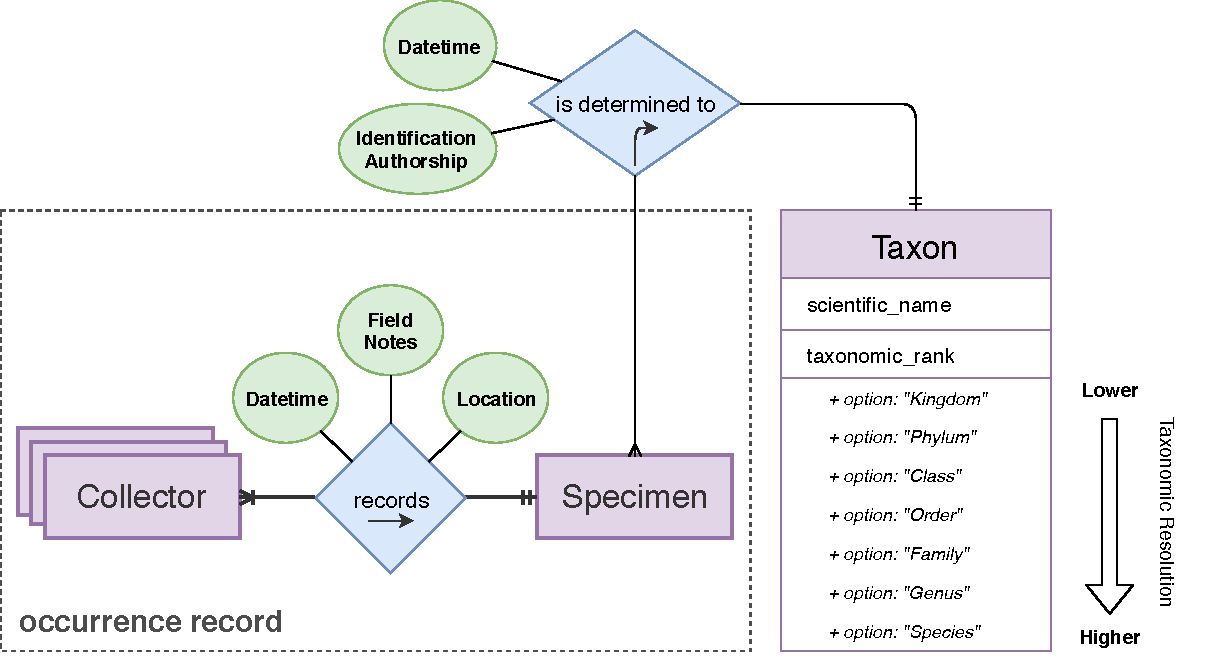
\includegraphics[width=\linewidth]{figures/collections_data/occurrences_er.pdf}
    \caption[Entity-relationship diagram illustrating the main features of species occurrence records]{Entity-relationship diagram illustrating the main features of species occurrence records. The cardinality of relationships is represented using the Crow's foot notation.}
    \label{fig:occurrences_er}
\end{figure}

%\clearpage


Over the last 40 years, many institutions have adopted digital database management systems---or in the simplest cases, electronic spreadsheets---for improving the management and accessibility of their specimens-related data~\cite{Sunderland2013}.
Occurrence-related information is digitally stored in relational databases, while keeping references to the physical vouchers.
Each row corresponds to an occurrence, and includes contextual information such as the collectors' names, the geographic coordinates, date and time of the occurrence and the taxonomic identity of the recorded specimen.
Some initiatives~(\textit{e.g.} Reflora\footnote{\url{http://reflora.jbrj.gov.br}}) have also devoted significant effort towards the large-scale digitalization of physical specimens from biological collections, making high-resolution photos of the specimens digitally available for researchers.

One important upside of storing species occurrence information digitally is that institutions can more easily replicate and share their data with others, thus supporting wide ranges of applications using biodiversity information \cite{Newbold2010}.
Some data aggregation initiatives, such as the Global Biodiversity Information Facility (GBIF), have provided technological solutions for serving data from multiple collections to researchers through programmatic and visual interfaces \cite{gbif}.
In this context, it becomes relevant to represent data in an standardized and interchangeable format, such that records from distinct collections can be more seamlessly integrated.

Darwin Core (DwC)\footnote{\url{http://rs.tdwg.org/dwc/}} is a body of standards designed to provide a consistent vocabulary for describing biodiversity-related information and making it exchangeable, accessible, reusable and interoperable \cite{Wieczorek2012}.
An extension of the Dublin Core Metadata Initiative~(DCMI)\footnote{\url{http://dublincore.org}}, DwC has been specifically created and adopted as a standard for publishing biodiversity data, composed of many terms to designate \textit{classes} of entities and their \textit{properties}.
The \textit{Occurrence} class includes terms for representing many aspects of the gathering act \textit{per se}, documenting the existence of organisms at particular places and times.
Taxonomic information of organisms is represented under the \textit{Taxon} class.
Throughout this chapter, we refer to darwin core terms by prepending `\textit{dwc:}' to names (\textit{e.g.} the \textit{Occurrence} class becomes \textit{dwc:Occurrence} and the \textit{Taxon} class, \textit{dwc:Taxon}).
However, the set of terms and definitions provided by DwC does not allow for the representation of semantic structures involving multiple classes of concepts.
The development of biodiversity \textit{ontologies}, which consist of domain-specific concepts, data and entities linked in an hierarchical structure, is a promising step towards overcoming such limitation \cite{Walls2014}.



% Species occurrence is not exclusive of biological collections Chapman2005b
%% Citizen science and informal collectors
% Hardisty2013
Last, it is worth noting that, although biological collections have been traditionally regarded as the main sources of species occurrence data, recent advances in mobile computing technology, associated with the increasing connectivity of electronic devices to the World Wide Web, have leveraged the participation of informal groups of nature observers towards recording and sharing biodiversity data in online platforms~\cite{Silvertown2009}.
Many of these communities also collaborate with researchers by sharing large amounts of records of their target organisms, in extents that would be otherwise impracticable to obtain, without enormous financial support.
The nature of such records is similar to those from biological collections in that they are punctual observations of specimens in nature, but also have some important distinctions.
First, nature observers usually materialize their observations through digital recordings~(audio, photo or video) instead of collecting physical biological samples.
The absence of physical specimens in many cases makes the identification of the observed organisms inaccurate, thus limiting the use of such data for scientific purposes.
In addition, identifications are often provided by a collaborative community of individuals with practical experience, not necessarily professional taxonomists and specialists.

\section{Limitations of data} 
\label{section:limitdata}
% Newbold2010 James2018 Hortal2007
% Presence vc presence-absence data
% Collectors Behavior (TerSteege2011)
% Limitations: sampling bias, lack of assessment of sampling effort, lack of geographic coverage
% Name ambiguity issue Groom2014

% Most species remain poorly collected , Nelson1990 TerSteege2011

% ===========
% Data issues
% -----------

Besides the remarkable relevance of biological collections as sources of biodiversity information, they are far from being adequate for investigating every aspect of natural systems.
This is partially a consequence of the fact that detailed information is unavailable or very scarce for most known organisms.
This scenario, referred to as the \textit{Wallacean Shortfall} \cite{Lomolino2004}, is even more critical for megadiverse countries, such as Brazil, which still remain largely unexplored for many regions and taxonomic groups \cite{Soberon2004}.
The lack of sufficient data for threatened species is even more concerning, as designing efficient programs for their conservation require knowledge on their geographic distribution and ecological requirements.
This shortage of data, combined with the non-systematic sampling and insufficient quality, limits the use of data from biological collections for many intended applications, many of which require an intensive amount of data to be available~\cite{Guisan2007}.
Failing to account for the inherent limitations of such data while posing and investigating their hypotheses, researchers may obtain erroneous or misleading results, eventually impacting the success of management policies that rely on such information \cite{Chapman2005}.
% Guisan2007 -> Many applications require high volumes of data, low sample size reduces the performance of many techniques
% Galante2017 -> Techniques for SDM using few records


\subsection{Sampling biases}
% charact. 2: Non-uniform sampling effort -> Lead to bias
One important aspect that often limits the usability of primary data from biological collections concerns the way in which it is gathered in the field.
In general, most species occurrence data composing biological collections derive from exploratory field expeditions, in which organisms are recorded in a non-systematic \textit{observational} fashion by different collectors, using different methods and at distinct circumstances (though records resulting from experimental studies are eventually incorporated in museums as well). 
As a result, the distribution of the sampling effort in such datasets is uneven and rarely quantified, leading to \textit{sampling biases}.

Building models without accounting for biases in data has been observed to strongly impact their performance, leading to spurious results which can be misinterpreted and, ultimately, lead to wrong decisions.
For instance, assessing patterns of species richness from species occurrence datasets has been shown to be particularly challenging due to geographical bias in data \cite{Hortal2007,Reddy2003}, as higher diversities tend to be observed at more accessible sites due to higher sampling effort.

As defined by \citeonline{Chrisman1991}, biases are uniform shifts in measured values, resulting from systematic errors that are introduced by some measurement system.
They are expressed as unrealistic tendencies in data, and can usually be mitigated with the adoption of random sampling designs.
%
Sampling bias in biodiversity data can be classified into several distinct categories, depending on the aspect of data under investigation \cite{Daru2017}.
Here we briefly present four of them, the first two (collector and taxonomic biases) being the most relevant in the scope of our work.
%
% collector bias, taxonomic bias, (geographic bias, trait bias, historical bias, seasonal bias) % Daru2017, Haripersaud2009 
\paragraph*{Collector bias.}
Not all collectors contribute to the same extent to biological collections.
In fact, it has been observed that a considerable percentage of records in biological collections are gathered by only a small subset of very productive collectors, while the vast majority of collectors contribute with just a few records each~\cite{Daru2017,Carine2012}.
This imbalance in the representativity of collectors is what defines the \textit{collector bias} in biological collections.
As the overall taxonomic composition of collections---as well as the geographical and temporal distribution of their records---tend to reflect the particular interests and collecting behavior of their most representative collectors, collector bias propagates to other categories of biases in the collection. Therefore, we consider that characterizing collector bias is a fundamental step towards understanding other types of biases.

\paragraph*{Taxonomic bias.}
Not all taxa are quantitatively represented in biological collections in the same proportions as they occur in natural systems.
Instead, the taxonomic composition of collections reflect the interests and collecting behavior of the communities of collectors contributing to them.
Moreover, rare species tend to be overrepresented in biological collections, as experienced collectors tend to prioritize collecting them over those which are more common \cite{Nelson1990}.
In addition, as collectors usually avoid collecting more than one exemplary of each species at the same place in a given expedition \cite{TerSteege2011}, common species tend to be underrepresented.
As the overall taxonomic composition of biological collections tend to reflect the interests and collecting behavior of their most productive collectors, taxonomic bias is intrinsically related to collector bias.
%
%Some studies have proposed to assess taxonomic bias of collectors by comparing the representativity of each taxon on their sets of records to the herbarium \cite{Haripersaud2009}. %Such approaches give at most a view of how well a collector represents the composition of the collection.
%However, if we consider the herbarium itself is composed of contributions of multiple collectors each with particular interests --- and therefore also biased ---, the herbarium is biased, not representing well the natural communities.
%As it is very common that collectors towards sampling the highest number of species as possible in localities they visit, the collection is non-random, and rare species tend to be overcollected and common species, undercollected \cite{TerSteege2011}.
%Biases of the most productive collectors would be hard to assess.

\paragraph*{Geographic bias.}
% [Kadmon, R., O. Farber, and A. Danin. 2004. Effect of roadside bias on the accuracy of predictive maps produced by bioclimatic models] 
Collection sites are not randomly selected in geographic space, nor they are all sampled to the same extent.
As features of the landscape make some areas more accessible for collection activities than others \cite{Hijmans2000}, collectors tend to prioritize those to maximize their productivity while minimizing costs.
Geographic bias thus arises as a consequence of non-uniform collecting effort in geographic space, and tends to reflect the preferred locations of the most productive collectors.
Some regions that are more accessible being thoroughly sampled (such as areas near urban centers, roadsides and margins of rivers);
while others that are more inaccessible, such as rainforests, being only poorly or not sampled at all.
%
Geographic bias is also observed at broader scales.
A compilation of the representativity of plants in GBIF by~\citeonline{Meyer2016} has shown that among the most representative countries and regions are the United States (mainly the west coast), Central America, countries in Europe (including the nordic countries), Australia, Japan, and New Zealand.


\paragraph*{Temporal bias.}
The patterns of the recording activities of collectors are not uniform over time.
Instead, collectors often show preferences towards performing field work in periods when they can get more productive, have more financial resources, or can find more organisms of their interests.
For instance, wet seasons possibly impact the performance of collectors in the field, and thus it would be natural to observe a relative drop on collecting activity during these periods.
Nevertheless, some organisms are better collected during wet periods~(such as \textit{Rivulidae} temporal fish), pushing collectors towards performing fieldwork despite unfavorable conditions.
Further, the availability of a naturalist for spending time in the field as a collector varies with their age, position, and stage in career.
While professional collectors would be available for collecting during weekdays, amateurs or students would be more available in weekends or vacation periods~\cite{Daru2017}.
The historical of records in biological collections therefore reflects the periods of activities of the most productive collectors.

% Two shortcomings: presence-only data and representativity


% Representativity
%Besides biases, another problem arising from non-uniform sampling effort concerns the representativity of species in biological collections.
%Collectors usually avoid collecting more than one exemplary of each species at the same place in the same expedition, and thus species representativity in museums do not correspond to their abundance in natural systems \cite{TerSteege2011}.
%In fact, rare species have been observed to be more represented than common ones due to the fact that more experienced collectors tend to prioritize collecting rare over common ones \cite{Nelson1990}.
%Moreover, non-uniform sampling effort hampers the assessment of species absences from `presence-only' occurrence data.
%As the sampling effort deployed over each location is usually not known for data in biological collections, the absence of a record for a species does not necessarily mean it does not occur there \cite{Graham2004}.
%Instead, it could be the case that no collectors who would potentially be interested on recording it have visited the location; or the species could not be detected at the time of the expedition.
% Problems in modeling
%Using presence-only data for assessing richness is problematic, although there are methods for overcoming this limitation, as most records available %for specimens are presence-only \cite{Zaniewski2002}.
%Richness was observed to be correlated to survey effort, richness is biased towards regions that are more thoroughly sampled \cite{Hortal2007}.

% Presence-only data and richness
%Non-uniform sampling effort also makes it hard to infer true absences from biological collection datasets.
%Species occurrence data is regarded as `presence-only', as they do not explicitly represent the absence of species.
%As the distribution of sampling effort towards locations is not known in biological collections, its data is regarded as `presence-only', which means that the absence of a record for a species at some location does not necessarily indicate that the species is truly absent \cite{Graham2004}.
%Instead, no collectors that would potentially be interested on recording it have visited the location.




% charact. 3: Data quality
% Briefly describe the limitations due to errors



\subsection{Data quality}
Besides biases, another important limitation in biological collection datasets concerns the \textit{quality} of data.
A definition for data quality (DQ) based on its \textit{fitness for the intended use} was first proposed in the context of geographical information systems \cite{Chrisman1984}, and became widely adopted by the BI community.
According to this definition, quality is not an absolute attribute of a dataset, but is rather given by its potential to provide users with valuable information, in specific contexts.
Assessing quality attributes of data is a fundamental step for any applications that might use it, and requires that users previously delimit the purpose, scope, and requirements of their investigation.
Data is considered to be of high quality if it is suitable for supporting a given investigation.
Depending on the application, users might need to improve the fitness of the data they have in hand, which is part of the data quality management process.

Loss of quality in biodiversity data can occur during multiple stages of its life cycle \cite{Chapman2005}, including the moment of the recording event, its preparation before it is incorporated in the collection, its documentation, digitalization, and storage.
% Include about data domains
Some of the most common problems are observed in the taxonomic and geospatial data domains, including the wrong identification of specimens, in part due to using outdated taxonomy; and bad georreferencing of records \cite{Soberon2004}.
In some cases, errors can be manually corrected by referring to supplementary information, such as the field notes of collectors \cite{Graham2004}.
However, this approach turns out impractical for large datasets, and methods for systematically assessing quality issues are required.


% Data problems
\citeonline{Dalcin2005,Veiga2014} have assessed the most common data quality issues in species occurrences datasets, and identified eight recurrent patterns of problems. %, observable across multiple data domains. 
During our study, we have identified five of them, which we considered to be most relevant:
(\textit{i})~\textbf{domain value redundancy}, when multiple distinct values in the dataset redundantly represent the same real-world entity;
(\textit{ii})~\textbf{non-atomic data values}, in case a value semantically contains multiple instances of the fundamental piece of information it should represent (an atomic value is regarded as being indivisible);
(\textit{iii})~\textbf{inconsistent data values}, in case they do not follow a strict standard, eventually leading to contradictory information;
(\textit{iv})~\textbf{incorrect data values}, when erroneous information are inserted in the dataset; and
(\textit{v})~\textbf{missing data value}, in case values at some field are absent (\textit{i.e.} null values).

A framework for systematically assessing and managing the ``fitness for use'' of biodiversity data from a user-centered perspective was recently proposed by \citeonline{KochVeiga2017}, and is based on three main components: \textbf{DQ Needs}, \textbf{DQ Solutions}, and \textbf{DQ Report}.
%
While defining DQ needs, users specify their \textit{use case}, comprising the main goals and scope of their investigation; the relevant \textit{information elements} that should be explicitly represented; and the \textit{dimensions} of data that should be assessed while measuring its quality.
Users also specify \textit{criteria} for defining acceptable measurements in each dimension; and activities for improving the suitability of data for the use case (\textit{enhancement}).
%
Within the scope of DQ solutions, users specify methods and implements tools for measuring, validating and enhancing data quality.
%
Finally, DQ reports are produced as documentations of the data quality assessment and management process in different contexts.
Users can therefore refer to such reports in order to evaluate whether their data is fit for their intended use, providing a basis for the collaborative development of data quality solutions (which authors refer to as a ``Fitness for Use Backbone'' (FFUB)).

\section{Data requirements for network modeling} % What should I do for improving data quality for SCN and CWN modeling
\label{section:datareq}
In this section, we briefly characterize aspects of data quality that are relevant for the network models presented in this dissertation.
Our models are constructed based on two \textbf{information elements}: the names of collectors and the taxonomic identity of the specimen at each occurrence record.
In a dataset following the DwC standards body, collector names and taxonomic identities should be found under the terms \textit{dwc:recordedBy} (class \textit{dwc:Occurrence}) and \textit{dwc:scientificName} (class \textit{dwc:Taxon}), respectively.
%
In SCNs, each record containing a set of collectors and a taxon. 
Interest ties are extracted from each record, linking each collector to the taxon.
More details on the construction process are provided in Section~\ref{subsec:scn-model-construction}.
%
In CWNs, only the collector field is required.
For each record, collaboration ties are created (or reinforced) by combining all collectors in a pairwise fashion.
More details of the construction process are provided in Section~\ref{section:cwn_construction_fromdata}.
%
Below we describe both information elements and highlight some of the main issues and requirements associated with them. 

% ========================================
% Information element: The collector field
% ----------------------------------------
\subsection{Collector names}\label{section:data_req_collector}
This information element contains the names of all collectors who were responsible for a species occurrence record.
In a DwC-compliant dataset, collectors names should be found under the term (or field) \textit{dwc:recordedBy} (within class \textit{dwc:Occurrence}), formatted as a list of collectors names concatenated into a string, using the vertical bar (` | ') as the delimiter.
For instance, a record authored by `M.A. Silva' and `N.T. Souza' would contain a string with value ``M.A. Silva | N.T. Souza''.
However, storing multiple names into a single string makes values in this field \textit{non-atomic}, thus requiring additional processing for the retrieval of individual names.

% names atomization
We refer to the process of extracting multiple names by splitting the string on a delimiter character as the \textbf{name atomization} routine, which is mandatory for our use case.
Applying the name atomization process to an entire dataset should be a trivial task if a consistent and non-conflicting delimiter (though not necessarily the vertical bar) is adopted throughout the entire dataset.
However, we suspect this is rarely the case for most species occurrence datasets.
Atomization issues arise when the atomization routine is unable to systematically distinguish names in a string, leading to the representation of unrealistic entities in the model.

% naming conventions
Using inconsistent (or ignoring) \textbf{naming conventions} while registering collectors names in a dataset is also potentially problematic, as it makes it more difficult to systematically interpret names and extract their component parts.
Naming conventions are rules used for shortening (or simplifying) names before they are inserted in the database.
One common practice is to abbreviate the first and middle names of collectors, while keeping the last name unabbreviated.
Under this convention, for instance, the name `João Souza Silva' would be mapped to `J.S. Silva'.
As collectors are not always aware of the naming convention adopted at the collection, they often include collectors names in their field notes using their own convention or, in the worse case, not using conventions at all.
The task to assure that all records are properly formated is therefore assigned to system managers, who must inspect and fix each entry manually before including them in the dataset.
As a result, names are eventually registered with typographical errors or being inconsistent with the adopted convention, although some database management systems are able to assist users in this aspect by parsing input names or by suggesting similar names that have already been registered.

% Heteronymous: result of inconsistent naming convention
Another negative effect of inconsistently formating collector names is the insertion of multiple \textbf{name variants} referring to the same real-world entity (domain value redundance).
This can also be the result of typos (e.g. souza becoming sousa), or simply omitting parts of the name (e.g. if there are two collectors, A.~M.~Souza and A.~P.~Souza, omitting the middle initial makes their names indistinguishable).
%
The \textbf{entity-resolution} problem concerns the mapping of name variants that refer to the same real-world entity.
\citeonline{Groom2014} came across the same problematic, considerable variations in the formats of names.
They used a name cleaning routine in which they merged all variants of names that could be unambiguously mapped to a single person, while excluding those which could not.
This problem was also tackled by \citeonline{EstevaoDaSilva2016} by using a data mining methodology, based on association rules analysis, for identifying possible name variants.

% Homonymous
Assuming that all records in a dataset are consistent with some naming convention and that they use the same character for delimiting names (\textit{i.e.}, names can be properly atomized), distinct real-world entities may still end up being registered under the same name.
These entities, which we refer to as being \textbf{homonymous}, are also problematic for our use case, as they are incorrectly represented in the network models as a single entity.
In case the naming convention requires the abbreviation of parts of the names, homonymous can be created in the database from two names that are originally distinct.
For instance, `João Souza Silva' and `Jorge Soares Silva' would be mapped to a homonymous `J.S. Silva', if both the first and middle names were abbreviated.
%
Some collections include mechanisms in their naming conventions for disambiguating homonymous.
For instance, a complementary field containing unique identifiers for collectors can be appended to each record in the dataset, allowing the identification and resolution of homonymous entities.
Also, suspect homonymous entities that are already introduced in the dataset can be screened by applying anomaly detection techniques to other collector-related fields.
For instance, an entity in the model displaying very improbable patterns of collecting activity (\textit{e.g.} activity peaks temporally spaced by 70 years) is likely to refer to multiple real-world entities.

% Omission
Finally, some collectors only include their own names in records in which they are first collectors, omitting the names of secondary collectors or, eventually, aggregating them under the expression `et al.'.
We refer to this issue as a \textbf{name omission} (within the \textit{completeness} DQ dimension), which strongly impacts as it fails to represent collaborative ties and collecting activities of the collectors who are not listed.

% Check Chapman2005a p.23

% ===================================
% Information element: The taxon name
% -----------------------------------
\subsection{Taxon name}
This information element contains the taxonomic identity assigned to the specimen from an occurrence record, being included into the taxonomic data domain.
In a DwC-compliant dataset, the taxonomic identities (or taxon) assigned to specimens at the highest resolution as possible are stored under the term \textit{dwc:scientificName}, which is part of the \textit{dwc:Taxon} class.
Other relevant elements within this class concern the common name of the taxon (\textit{dwc:vernacularName});
the rank of the taxon (\textit{dwc:taxonRank}); 
the names of higher-rank taxa within which the the taxon is classified (\textit{dwc:kingdom}, \textit{dwc:phylum}, \textit{dwc:order}, \textit{dwc:family}, \textit{dwc:genus}, \textit{dwc:specificEpithet});
the name of the author of the scientific name of the taxon\footnote{not to be confused with the author of the identification, in \textit{dwc:identifiedBy} (\textit{dwc:Identification} class).} (\textit{dwc:scientificNameAuthorship}).
%
Two important dimensions that possibly impact the fitness of taxonomic information for our use case concern the \textit{accuracy} and \textit{precision} of identifications; as well as \textit{misspelling errors}.

As exposed by \citeonline{Chapman2005a}, the \textbf{accuracy of taxonomic identifications} depends on the level of expertise of the professionals providing them.
For instance, a determination of taxonomic identity can be provided by the collector; by a professional taxonomist who is not an expert in the taxonomic group; or by a professional taxonomist who is either a regional or world specialist in that group.
Determinations provided by experts are, in general, more credible than those by non-experts, though even experts cannot always guarantee the highest degree of certainty on every identification.
Although information about the level of expertise of the determiners is typically not included in datasets from biological collections, many institutions adopt nomenclatural terms to convey the level of certainty in identifications, for instance `aff.' (for \textit{`affinis'}, suggesting affinity but not necessarily identity to other taxon) or `cf.' (for \textit{`confer'}, which is usually placed between the genus and epithet in the name of a species, indicating an uncertainty in the identification due to technical difficulties).

\textbf{Misspelling errors} are also included in the accuracy dimension of taxonomic data quality \cite{Veiga2014}, and are introduced in the datasets in a variety of ways, including typographic errors (typos), encoding issues, and from the incorrect transcription of names from how they sound \cite{Dalcin2005}.
Taxonomic authority files (files containing accepted taxonomic names) have been widely used for preventing the insertion of new invalid names during data entry; or for checking the validity of names already included in databases \cite{Chapman2005a}.
In addition, \citeonline{Dalcin2005} has proposed the use of both phonetic and string similarity algorithms for automatically screening potential spelling errors, by matching pairs of slightly different names with high degrees of similarity.
Further development towards this direction has led to the development of \textit{Taxamatch} algorithm, having achieved remarkable results \cite{Rees2014a}. 

The \textbf{precision dimension of taxonomic data} is related to the most specific rank at which a specimen can be identified, \textit{i.e.}, its taxonomic resolution \cite{Veiga2014}.
Depending on the modeling requirements, a minimal taxonomic resolution may be necessary for the construction of the networks, making datasets more or less adequate for use.
Some applications using our models might require the representation of taxa at higher taxonomic resolutions  (\textit{e.g.} at the level of species), whereas for others it could suffice to use lower resolutions, such as the family level.
The precision of identifications is also related to the level of expertise of the determiners, although some groups of organisms are naturally more difficult to identify than others.
For instance, identifying mammals to the rank of species is far easier than insects.
Furthermore, higher levels of expertise are often required for identifying organisms within larger families, which comprise a higher number of species.
%
Therefore, assessing the proportion of records in a dataset that qualify for our network-based approach requires first defining the taxonomic resolution to be adopted during modeling.
In that sense, the \textbf{completeness of taxonomic information} (the proportion of records that are usable) is intrinsically associated with data precision.

Last, there are cases in which a taxon is referred to by to distinct names, although only one of them is accepted at any given time, according to the \textit{code of nomenclature} adopted.
Such names are said to be \textbf{synonyms}, and are an example of the domain value redundancy problem in the taxonomic data domain.
Similarly to redundancies in collector names, this issue leads to semantic inconsistencies in the network models (more especifically in SCNs), with entities represented more than once.
The insertion of synonyms in datasets can also be avoided during the data entry process, by using authority files based on the current code of nomenclature \cite{Veiga2014}. 













%% As it is common practice for botanists to record each species once during field work, some important ecological attributes such as the species abundance are not to be directly inferred from such data. {check van Gemerden 2005, from Haripersaud2009}


% Biological collections are composed of aggregates of multiple biodiversity surveys, each recorded with particular methodologies
% Records sampled using distinct methodologies can be combined for optimizing data use \cite{VanGemerden2005}.











% ============
% Data quality
% ------------
% [Soberon2004]

% Data quality among collection records is uneven -> worse for large datasets and for datasets composed by multiple sources
% Procedures are needed for correcting problems

% Quality issues: 
%% Determination issues: many specimens are incorrectly identified;
%% outdated taxonomy;
%% georreferencing errors.

% Data atomicity issues:
% Some fields are not atomic: more than one entity is represented as a single data element. 
% In the recordedBy field, Darwin Core standards state that distinct names should be separated by | (delimiter).
% This varies depending on the standard a collection uses. For example, the BRAHMS system recommends using a ';' as the delimiter.
% BRAHMS docs: https://herbaria.plants.ox.ac.uk/bol/brahms/support/documentation

% Identity issues:
% Entities are not guaranteed to have the same ids through distinct datasets.
% Even in the same datasets there may be variations in their names
% this is specially problematic for fields like the collectors field, which is overlooked for most applications of such data. 
% Some standards provide guidelines for including collectors names: last name + first initials...
% However different standards give distinct guidelines and thus name variants are common.
% How to map all name variants to the same entity? -> This leads to the Entity-resolution problem


% Data fit for use


% =============
% Data cleaning
% -------------
%[Chapman2005a]

% Why do we need data cleaning? -> We must make data fit for its indended use

% Goal: improving data quality, removing or treating entries that are 

% Adopting standardized collectors names
% Checking collectors itineraries -> look for the spatial pattern of records by the collector


% ================
% References
% ----------------
%% Museum-based informatics{Graham2004}



